\documentclass{beamer}
\usetheme{Madrid}

\usepackage[utf8]{inputenc}
\usepackage[T1]{fontenc}
\usepackage{graphicx}

\title[Projet Programmation Imp]{Présentation Projet Programmation Impérative}

\author[G.Percet, N.Volianskyi, M.Melkonian]{Percet Gauthier \and Nikita Volianskyi \and Mark Melkonian}

\date{}

\begin{document}

	\begin{frame}[plain]
		\maketitle
	\end{frame}

	\begin{frame}{Sommaire}
		\tableofcontents
	\end{frame}

	\section{Introduction}
	\begin{frame}{Introduction}
		\begin{itemize}
			\item Dans le cadre du projet de programmation impérative, nous avons réalisé une implémentation de l'algorithme des K plus proches voisins (KPPV).
			\item L'objectif de ce projet était de réaliser un programme complet permettant d'exécuter l'algorithme des KPPV avec deux types de structures de données.
			\item Nous avons utilisé pour cela le langage C, la bibliothèque MLV, Python et Bash.
		\end{itemize}
	\end{frame}

	\section{Architecture du code}
	\begin{frame}{Organisation des modules et répartition du travail}
		\begin{block}{Structure du projet}
			\begin{itemize}
				\item \textbf{main.c} : Point d'entrée, mesures de performance et sauvegarde des résultats.
				\item \textbf{interface.c} : Gestion de l'affichage graphique (MLV).
				\item \textbf{tree\_kd.c} : Implémentation de la recherche KPPV par arbre KD.
				\item \textbf{points\_list.c} : Implémentation de la recherche KPPV par liste (force brute).
				\item \textbf{vector.c / point.c} : Structures de données de base.
				\item \textbf{test.sh / graphique.py} : Automatisation des tests et génération des graphiques.
			\end{itemize}
		\end{block}
	\end{frame}

	\section{Analyse des graphiques}

	\begin{frame}{Variation de k (liste vs arbre)}
		\begin{columns}
			\column{0.5\textwidth}
				\IfFileExists{../results/vary_k/graph_list.png}{
					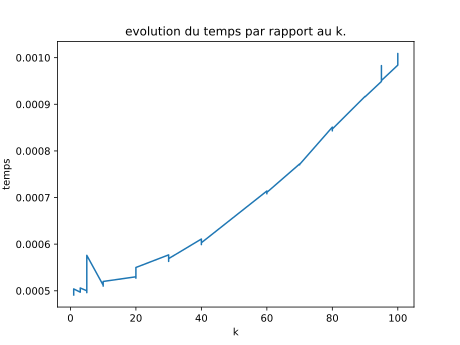
\includegraphics[width=\textwidth]{../results/vary_k/graph_list}
				}{\textit{(lancer test.sh)}}
			\column{0.5\textwidth}
				\IfFileExists{../results/vary_k/graph_tree.png}{
					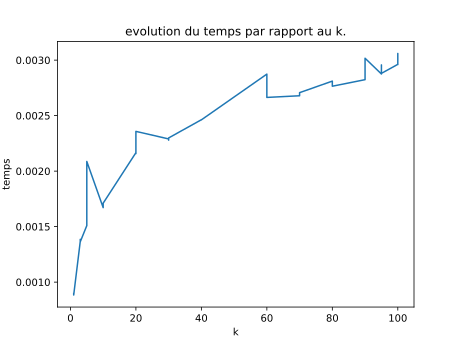
\includegraphics[width=\textwidth]{../results/vary_k/graph_tree}
				}{\textit{(lancer test.sh)}}
		\end{columns}
	\end{frame}

	\begin{frame}{Variation des dimensions (liste vs arbre)}
		\begin{columns}
			\column{0.5\textwidth}
				\IfFileExists{../results/vary_dim/graph_list.png}{
					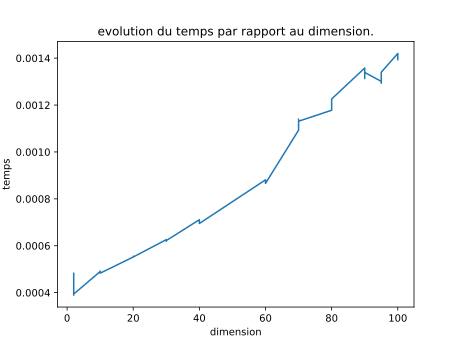
\includegraphics[width=\textwidth]{../results/vary_dim/graph_list}
				}{\textit{(lancer test.sh)}}
			\column{0.5\textwidth}
				\IfFileExists{../results/vary_dim/graph_tree.png}{
					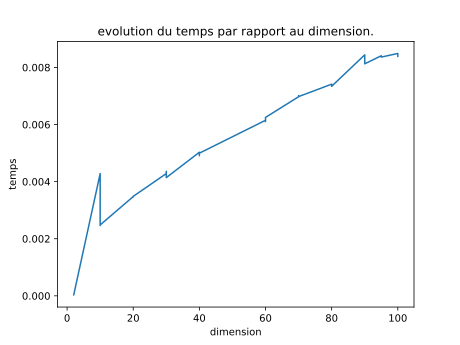
\includegraphics[width=\textwidth]{../results/vary_dim/graph_tree}
				}{\textit{(lancer test.sh)}}
		\end{columns}
	\end{frame}

	\begin{frame}{Variation du nombre de points (liste vs arbre)}
		\begin{columns}
			\column{0.5\textwidth}
				\IfFileExists{../results/vary_nb_points/graph_list.png}{
					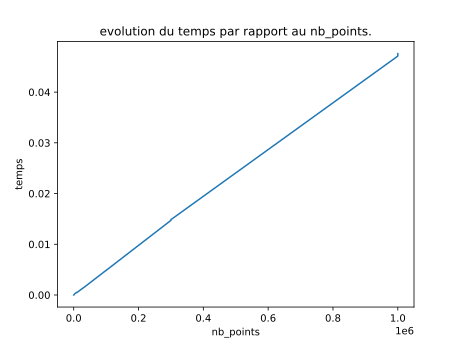
\includegraphics[width=\textwidth]{../results/vary_nb_points/graph_list}
				}{\textit{(lancer test.sh)}}
			\column{0.5\textwidth}
				\IfFileExists{../results/vary_nb_points/graph_tree.png}{
					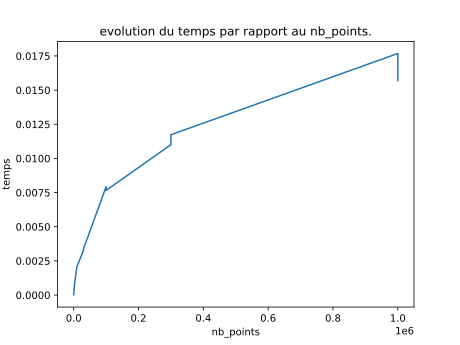
\includegraphics[width=\textwidth]{../results/vary_nb_points/graph_tree}
				}{\textit{(lancer test.sh)}}
		\end{columns}
	\end{frame}

	\section{Conclusion}
	\begin{frame}{Conclusion}
		\begin{itemize}
			\item Bilan des fonctionnalités implémentées.
			\item Difficultés rencontrées et solutions apportées.
			\item Perspectives d'amélioration.
		\end{itemize}
	\end{frame}

\end{document}
